\clearpage
\section{Foundation\label{sec:foundation}}

This chapter presents the theoretical and technical background underlying the proposed AI-assisted process guidance system. It introduces \gls{llm} and Retrieval-Augmented Generation (RAG) as the core technological concepts. Furthermore, relevant aspects of knowledge representation in industrial maintenance and essential principles of system architecture are outlined. These foundations provide the basis for the methodology and system design described in the following chapters.

\subsection{LLMs - Large Language Models\label{sec:LLM}}
Large Language Models (LLMs) are advanced deep learning models designed to understand and generate natural language by learning statistical patterns from large-scale text corpora. Most contemporary LLMs are based on transformer architectures, which enable the modeling of contextual dependencies across long text sequences. Through large-scale pre-training and subsequent task adaptation, these models can perform a range of natural language processing tasks, including question answering, summarization, and semantic retrieval. In industrial and manufacturing contexts, LLM-based systems have been investigated to support knowledge sharing and operational assistance. For example, LLM-powered tools have demonstrated their ability to retrieve domain-specific information and assist users in navigating complex technical documentation  \cite{freire_knowledge_2024}. Similarly, implementations aimed at enterprises show that LLMs can support question answering from various organizational knowledge bases, improving access to dispersed information sources \cite{sahin_llm_2024}.

Despite their strong generative capabilities, LLMs primarily rely on parametric knowledge encoded during training, which may not always reflect current or proprietary industrial data. Research on the use of LLMs for information retrieval shows both their potential and limitations when used alone for precise knowledge access tasks \cite{zhu_large_2026}.
To address these constraints, recent work in industrial knowledge management proposes retrieval-augmented approaches that integrate external document retrieval with generative reasoning, thereby improving factual grounding and contextual accuracy \cite{chen_application_2025}.
Also, research on the integration of LLMs and other technologies like augmented reality has revealed the potential of LLMs in facilitating contextualized maintenance and even interactive industrial assistance \cite{angelopoulos_industrial_2025}. Such advancements in the application of LLMs underscore the importance of LLMs in the context of industrial environments. In order to understand the mechanisms through which LLMs have been able to realize such potential and importance, it is critical to understand the basic architecture of LLMs, which is based on the Transformer architecture.
\subsubsection{Transformer Architecture\label{sec:Transformer}}
The Transformer architecture is the foundation of modern \gls{llm} and represents a major advancement in the field of \gls{nlp}) \cite{vaswani2017attention}. Unlike earlier neural network approaches that relied on \gls{rnns} or \gls{cnns}, the Transformer introduces a self-attention mechanism that allows the model to evaluate relationships between all tokens within a sequence simultaneously. This mechanism enables the model to capture long-range dependencies in textual data more effectively. Traditional architectures such as \acrshort{rnns} and \acrshort{lstms} process sequences step by step, which can limit efficiency when handling long inputs. In contrast, the Transformer processes the entire input sequence in parallel, resulting in significantly improved computational efficiency and scalability \cite{vaswani2017attention}.

\begin{figure}[H]
    \centering
    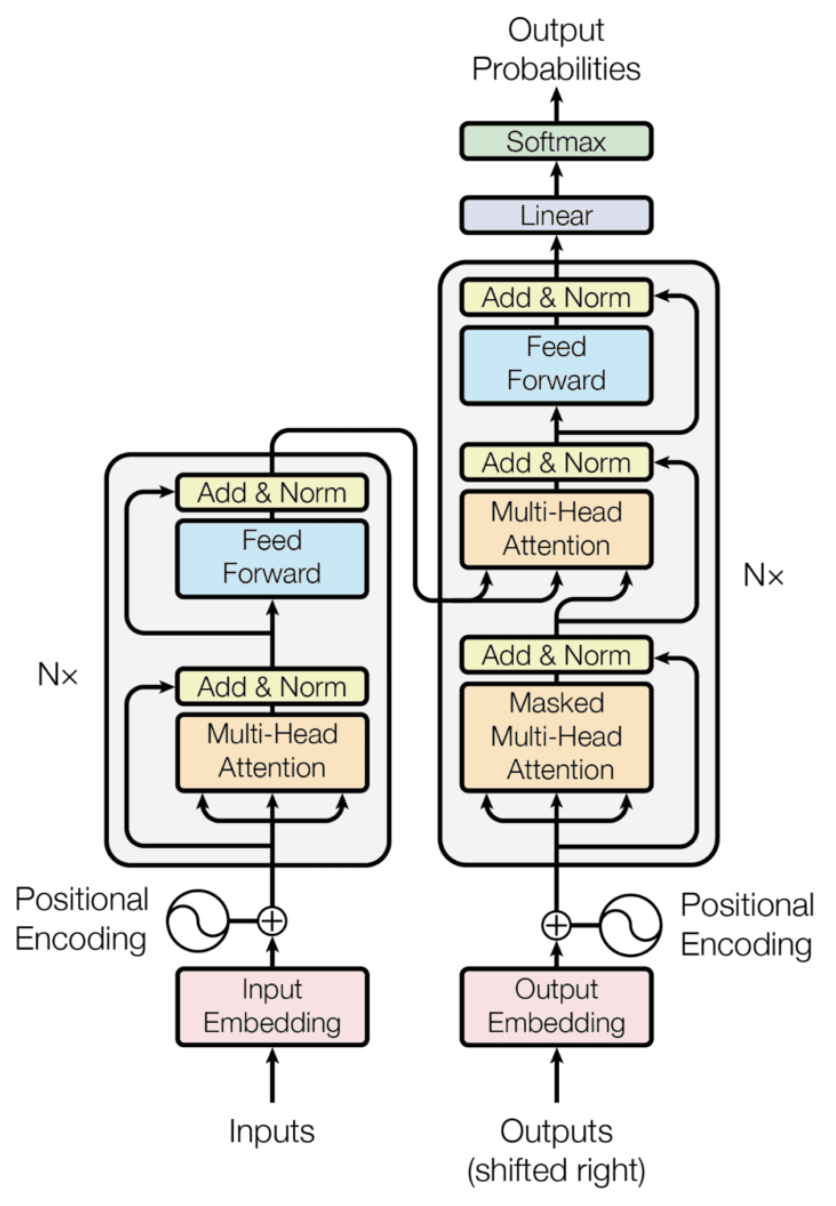
\includegraphics[width=0.8\textwidth, height=8cm, keepaspectratio]{images/Transformer Architecture.png}
    \caption[Transformer Architecture Overview]{Transformer Architecture Overview \cite{vaswani2017attention}}
    \label{fig:transformer_architecture}
\end{figure}
Figure \ref{fig:transformer_architecture} illustrates the overall structure of the Transformer model introduced by \cite{vaswani2017attention}. The architecture follows an encoder–decoder design composed of multiple stacked layers. The encoder processes the input sequence and transforms it into contextual representations, while the decoder uses these representations to generate the output sequence. Each encoder layer contains two main components: a multi-head self-attention mechanism and a position-wise feed-forward neural network. Residual connections and layer normalization are applied after each sub-layer to stabilize training and improve gradient flow.
A key component of the Transformer architecture is the attention mechanism, particularly multi-head self-attention. This mechanism enables the model to focus on different parts of the input text simultaneously and to learn various contextual relationships between words. During training, tokens are first converted into numerical representations known as embeddings, which capture semantic relationships in vector space. Positional encodings are then added to these embeddings to retain information about the order of tokens within a sequence. Through multiple stacked layers of attention and feed-forward networks, the Transformer progressively refines these representations, enabling the model to learn complex linguistic patterns and contextual dependencies \cite{vaswani2017attention}.

Because of their scalability and ability to capture contextual relationships effectively, Transformer-based architectures have become the primary design paradigm for modern \gls{llm} such as GPT, BERT, and other generative language systems. These architectures enable models to be trained on extremely large datasets, allowing them to perform a wide range of language understanding and text generation tasks through natural language prompts. The resulting capabilities form the technological basis for advanced applications, including knowledge retrieval systems, conversational agents, and AI-supported decision-making tools. Consequently, understanding the Transformer architecture is crucial for explaining how LLMs interpret and generate language. This understanding also provides the foundation for approaches such as retrieval-augmented generation, which enhance model responses by incorporating information from external knowledge sources to produce more reliable and contextually grounded outputs \cite{vaswani2017attention}.

\subsubsection{Pre-training and Instruction Tuning \label{sec:Pre-training and Instruction Tuning}}
\gls{llm} are developed using a multi-stage training process, which includes pre-training followed by fine-tuning or instruction tuning. In the pre-training stage, the model is trained using large-scale text data collected from a variety of sources, such as books, websites, and scientific publications \cite{devlin2019bertpretrainingdeepbidirectional}.
The goal of this stage is to understand general linguistic structures, contextual relationships, and semantic representations in natural language \cite{devlin2019bertpretrainingdeepbidirectional}.

Pre-training is commonly conducted using self-supervised learning objectives, where the model learns by predicting missing or next tokens within a sequence. This type of training allows the model to be trained on language patterns without the need for any labeled datasets. As a result, the model acquires a broad understanding of language that can later be transferred to downstream tasks \cite{devlin2019bertpretrainingdeepbidirectional}. Large pre-training has also been demonstrated to enable models to carry out different natural language processing tasks using natural language prompts with minimal task-specific training data \cite{brown2020languagemodelsfewshotlearners}.

After the pre-training stage, models are typically fine-tuned for specific tasks by additional training on smaller, domain-specific datasets. This fine-tuning process enables the model to optimize its parameters for improved performance on targeted tasks such as question answering, text classification, or dialogue generation \cite{brown2020languagemodelsfewshotlearners}. In the context of \gls{llm}, fine-tuning \cite{kelly2023gpt35finetuning} plays a critical role in adapting general-purpose models to specialized domains, including enterprise knowledge systems and industrial applications \cite{llmfinetuning2024}.

More recently, instruction tuning has been introduced to improve the usability of LLMs in interactive environments. Instruction tuning trains models on curated instruction–response pairs so they learn to follow natural-language instructions and produce responses aligned with user queries \cite{ouyang2022traininglanguagemodelsfollow}. In addition, reinforcement learning from human feedback (RLHF) has been used to refine model outputs further and improve alignment with human expectations \cite{ouyang2022traininglanguagemodelsfollow}.

Pre-training, fine-tuning, and instruction tuning collectively constitute the foundation of modern Large Language Model (LLM) development. These strategies enable models to acquire general linguistic patterns during large-scale training and subsequently adapt to a variety of downstream tasks through natural language prompts \cite{brown2020languagemodelsfewshotlearners}. Instruction tuning and reinforcement learning further enhance the capacity of \gls{llm} to follow user instructions and generate responses that align with human intent\cite{ouyang2022traininglanguagemodelsfollow}. Consequently, LLMs are applied to a broad range of tasks, including conversational systems, information retrieval, and knowledge assistance tools\cite{brown2020languagemodelsfewshotlearners}. In knowledge-intensive fields such as engineering and industrial operations, fine-tuning techniques facilitate the adaptation of general-purpose language models to domain-specific datasets, there by enabling intelligent systems that assist users in accessing and interpreting complex technical information \cite{llmfinetuning2024}.

\subsubsection{Capabilities of LLMs\label{Capabilities of LLMs}}
Large Language Models (LLMs) demonstrate strong capabilities for understanding and generating natural language across a range of tasks\cite{chowdhery2022palmscalinglanguagemodeling}. Through large-scale pre-training on diverse text corpora, these models learn contextual connections between words\cite{Guo_2021}. They can perform tasks such as text generation, summarization, translation, and question answering using natural language prompts\cite{brown2020languagemodelsfewshotlearners}. Additionally, LLMs exhibit few-shot and zero-shot learning abilities, allowing them to adapt to new tasks based on instructions or examples provided within prompts\cite{brown2020languagemodelsfewshotlearners}.

Instruction tuning helps \gls{llm} to understand better and follow natural-language instructions, leading to more effective human-AI interaction \cite{ouyang2022traininglanguagemodelsfollow}. Fine-tuning also lets these models adapt to specific domains by training them on specialized datasets\cite{llmfinetuning2024}. Because of these features, \gls{llm} work well for tasks that require handling and analyzing large amounts of text.


\subsection{RAG - Retrieval Augmented 
Generation\label{sec:RAG}}
\acrfull{rag} is an approach that integrates information retrieval with the generative capabilities of traditional \acrfull{llm}, which generate responses solely based on knowledge acquired during training, which is constrained by the data available at that time. Consequently, these models usually lack access to current, proprietary, or domain-specific information. RAG overcomes this drawback by enabling language models to retrieve relevant information from external knowledge sources during response generation \cite{IBM2023RAG}. The retrieved material serves as contextual input, guiding the model to produce more accurate, grounded responses. Due to its capacity to combine external knowledge with generative reasoning, RAG has developed as a significant architectural strategy for developing knowledge-intensive AI systems and enterprise knowledge management solutions \cite{WikipediaRAG2024}\cite{Holvoet2025RAG}.

\subsubsection{Embeddings and Vector Representations \label{sec:Embeddings and Vector Representations}}
Retrieval-based artificial intelligence systems transform textual data into numerical representations known as embeddings. These embeddings represent words, sentences, or documents as high-dimensional vectors to capture semantic relationships within texts \cite{chen_application_2025}. Representing text as vectors through embeddings enables systems to assess semantic similarity between pieces of information, resulting in more effective information retrieval than traditional keyword-based search methods \cite{Holvoet2025RAG}

Embedding models are trained on large text corpora to learn contextual relationships between words and phrases. As a result, semantically related concepts are represented by vectors positioned close to each other in the embedding space \cite{chen_application_2025}.
In industrial maintenance contexts, terms such as “crane fault diagnosis” and “lifting equipment malfunction” can be represented as vectors that are close to each other, even though they do not share identical keywords. This approach enables retrieval systems to identify relevant documents based on semantic similarity rather than relying solely on exact word matching \cite{Rusum2024VectorDB}.

Formally, a text input $T$ can be represented as a vector in a $d$-dimensional embedding space:
\[
T \rightarrow \mathbf{v} \in \mathbb{R}^{d}
\]
where $d$ denotes the dimensionality of the embedding vector. These vector representations are the basis of semantic retrieval in modern \acrshort{ai} systems. Retrieval-augmented architectures, for example, use embeddings to extract relevant information from large document collections \cite{chen_application_2025}.

\subsubsection{Vector Databases and Similarity Search\label{sec:Vector Databases and Similarity Search}}
Once textual data is transformed into embeddings, these vectors must be stored and efficiently retrieved when users submit queries. Vector databases are specialized database systems designed to manage high-dimensional vector representations and support similarity-based search operations \cite{Holvoet2025RAG} . Unlike traditional relational databases that depend on exact keyword matching, vector databases support semantic retrieval by comparing vector representations \cite{Rusum2024VectorDB}.

During the retrieval process, the system converts a user query into an embedding using the same embedding model that represents the database documents. The system subsequently compares the query vector with stored document vectors in order to identify the most semantically similar entries \cite{chen_application_2025}. This comparison is commonly performed using similarity metrics such as cosine similarity, which measures the angle between two vectors:
\[
\text{cosine similarity}(A,B) = \frac{A \cdot B}{\|A\|\|B\|}
\]
where $A$ and $B$ represent vector embeddings. A similarity score closer to 1 indicates a stronger semantic relationship between the two vectors, while values closer to 0 indicate lower similarity \cite{Rusum2024VectorDB}.

For example, when a maintenance engineer searches for “hydraulic crane pressure issue”, the vector database may retrieve documents related to “hydraulic pressure faults in lifting equipment” even if the exact keywords differ. This ability to retrieve semantically related information is essential in knowledge-intensive systems such as \acrfull{rag}, in which retrieved documents provide contextual information to the language model \cite{chen_application_2025} \cite{Holvoet2025RAG}.
\subsubsection{RAG Pipeline Architecture\label{sec:RAG Pipeline Architecture}}
\autoref{fig: General architecture of a Retrieval-Augmented Generation pipeline} illustrates the architecture and functioning of the RAG framework.

\begin{figure}[H]
    \centering
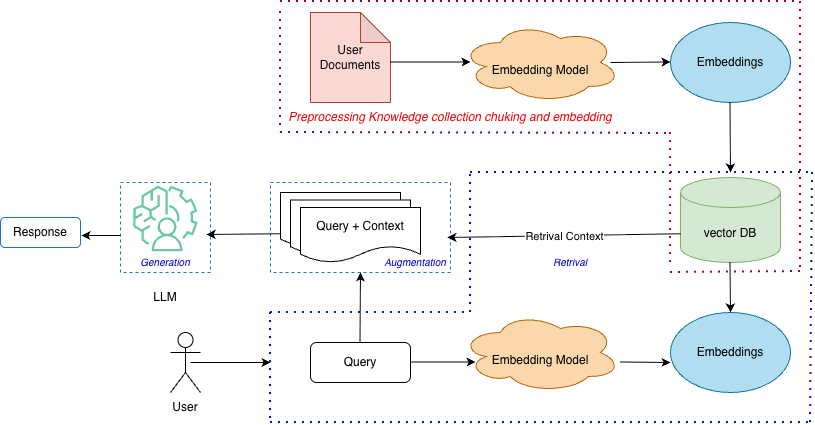
\includegraphics[width=0.8\textwidth, height=8cm, keepaspectratio]{images/RAG Pipeline.drawio.png}
    \caption[General architecture of a Retrieval-Augmented Generation pipeline]{General architecture of a Retrieval-Augmented Generation pipeline \cite{sahin_llm_2024}}
    \label{fig: General architecture of a Retrieval-Augmented Generation pipeline}
\end{figure}

As shown in \autoref{fig: General architecture of a Retrieval-Augmented Generation pipeline}, the \acrfull{rag} architecture consists of several interconnected stages that combine information retrieval with language model generation. These stages include accessing information sources, processing user queries, retrieving relevant document segments from a knowledge base, and generating responses using a large language model \cite{sahin_llm_2024}. Together, these components enable the system to retrieve relevant knowledge and produce contextually grounded responses.

The \gls{rag} pipeline operates through a series of stages, starting with the preparation of knowledge sources and concluding with the generation of a response based on retrieved contextual information. The primary stages of this process are outlined below.

\begin{enumerate}[label=\textbf{\arabic*.}]
    \item \textbf {Knowledge Source Preparation}
    
    The pipeline begins with a collection of domain documents, such as manuals, reports, or knowledge base entries, that serve as information sources for the system \cite{sahin_llm_2024}

    
    \item \textbf{Text Processing and Embedding Generation}
    
    The documents are divided into smaller text segments. These segments are then converted into numerical vector representations called embeddings that capture the semantic meaning of the text \cite{sahin_llm_2024}\cite{Holvoet2025RAG}.
    \item \textbf {Storage in a Vector Database}
    
    Once embeddings are generated, they are stored in a vector database \cite{Holvoet2025RAG} designed for efficient similarity-based retrieval. Such databases facilitate rapid searches within extensive collections of embeddings and enable the identification of relevant document segments in response to specific queries \cite{Rusum2024VectorDB}.
    \item \textbf {Query Encoding}

    When a user submits a query, the system processes the input and converts the query into a vector embedding using the same embedding model used for the documents. This ensures that both the query and the stored documents reside in the same vector space, enabling effective similarity comparisons \cite{sahin_llm_2024}.
    \item \textbf {Similarity-Based Retrieval}

    The query embedding is compared with the stored embeddings in the vector database to retrieve the most relevant document segments. This retrieval step typically uses similarity metrics such as cosine similarity (see section ~\ref{sec:Vector Databases and Similarity Search}) and returns the top-ranked document fragments that are most semantically related to the query 
    \cite{Rusum2024VectorDB}
    \item \textbf {Context Augmentation}

    Retrieved document segments are integrated with the original user query and supplied to the large language model as contextual input. This process enables the model to access relevant background information from the knowledge base prior to response generation \cite{sahin_llm_2024}. Incorporating retrieved content into the prompt allows the model to ground its reasoning in external knowledge, rather than relying exclusively on information encoded during training. Consequently, the generated response is more likely to be factually accurate and consistent with the retrieved documents \cite{chen_application_2025}.

    \item \textbf {Response Generation}
    
    In the final stage, the large language model generates a response using both the user query and the retrieved contextual information. The model processes this combined input to produce a coherent and informative answer that accurately reflects the relevant knowledge from the document collection \cite{sahin_llm_2024}. Integrating retrieval with language generation enables \acrfull{rag} systems to deliver responses that are more precise, contextually relevant, and consistent with the available knowledge sources \cite{chen_application_2025}.
\end{enumerate}

\subsection{Knowledge Representation in Industrial Maintenance \label{sec:Knowledge Representation in Industrial Maintenance}}

\subsubsection{structured vs Unstructured Data \label{sec:tructured vs Unstructured Data}}

\subsubsection{Maintenance Manuals and Documentation \label{sec:Maintenance Manuals and Documentation}}

\subsubsection{Chunking and Knowledge Extraction \label{sec:Chunking and Knowledge Extraction}}

\subsection{Decision Support Systems \label{sec:Decision Support Systems}}

\subsubsection{Rule-Based Systems \label{sec:Rule-Based Systems}}

\subsubsection{AI-Based Decision Support \label{sec:AI-Based Decision Support}}

\subsubsection{Limitations of Traditional Approaches\label{sec:Limitations of Traditional Approaches}}


\subsection{Process Guidance in Industrial Systems \label{sec:Process Guidance in Industrial Systems}}

\subsubsection{Maintenance Processes \label{sec:Maintenance Processes}}

\subsubsection{Challenges in Knowledge Access \label{sec:Challenges in Knowledge Access}}

\subsubsection{Digital Assistance Systems \label{sec:Digital Assistance Systems}}


\subsection{System Architecture Concepts Systems \label{sec:System Architecture Concepts}}

\subsubsection{Client–Server Architecture \label{sec:Client–Server Architecture}}

\subsubsection{API-Based LLM Integration \label{sec:API-Based LLM Integration}}

\subsubsection{Data Storage and Traceability \label{sec:Data Storage and Traceability}}

\subsection{Data Formats and Interoperability \label{sec:Data Formats and Interoperability}}

\subsubsection{JSON \label{sec:JSON}}

\subsubsection{REST APIs\label{sec:AREST APIs}}

\subsubsection{Logging and Metadata \label{sec:Logging and Metadata}}

